\documentclass[12pt]{ctexart}
\usepackage{amsfonts,amssymb}
\usepackage{float}
\usepackage{graphicx}
\usepackage{amsmath}
\usepackage{listings}
\usepackage{geometry}
\usepackage[usenames,dvipsnames]{xcolor}
\usepackage{setspace}
\geometry{a4paper}
\geometry{top=2cm} 
\geometry{bottom=2cm}
\geometry{left=0.5cm}
\geometry{right=1cm}

\title{微分方程数值解~上机作业 1}
\author{凌子恒 \\ 信息与计算科学 3200102551}

\begin{document}

\maketitle

\subsection{原理分析}

利用有限差分法求解二维 Poisson 方程。

设点 $(ih,jh)$ 处点值为 $u_{i,j}$。

对于 regular point $(ih,jh)$,以 $-\dfrac{4u_{i,j}-u_{i+1,j}-u_{i-1,j}-u_{i,j+1}-u_{i,j-1}}{h^2}$ 作为 $\Delta u$ 估计。

对于 irregular point $(ih,jh)$,分别计算 $x,y$ 上二阶导。以 $x$ 方向上有非规则边界 $((i+\theta)h,jh)$ 为例,设其点值为 $u'$,以 $\dfrac{2((1+\theta)u_{i,j}-u'-\theta u_{i-1,j})}{\theta(1+\theta)h^2}$ 作为二阶导估计。其余情况可类似处理。

对于边值 $(ih,0)$ 处的一阶导,以 $\dfrac{3u_{i,0}-2u_{i,1}+u_{i,2}}{2}$ 近似。其余边值也同理。

\subsection{代码解释}

定义 solution 类存放结果。

solution 类有两个构造函数,分别对应 $(0,1)^2$ 和 $(0,1)^2-D$。

两个构造函数的前三个参数均为:Possion 方程等式右侧函数 $f$,边值函数,以及格点段数。

其中边值函数期待返回类型为 pair<int,double>,其中第一项为 $1$ 表示给出的是边界处的一阶导,为 $0$ 表示给出的是边值。所有一阶导均给出垂直边界的方向导数,其中方向向内。

对于第二个构造函数,还需要按顺序给出 $D$ 的圆心 $x,y$ 坐标及半径。

构造完成后,可以调用 operator() 求出某个点的估计函数值。对于不规则区域,可以调用 is\_domain() 函数得到需要求值的点是否在定义域内。

利用定义了的 norm 函数可以计算出范数。

\subsection{具体例子(题 2)}

$u=e^{y+\sin x}\Rightarrow \begin{cases}
	u_x=(\cos x)e^{y+\sin x}\\
	u_y=e^{y+\sin x}
\end{cases}\Rightarrow \begin{cases}
	u_{xx}=(\cos^2 x)e^{y+\sin x}-(\sin x)e^{y+\sin x}=e^{y+\sin x}(1-\sin x-\sin^2 x)\\
	u_{yy}=e^{y+\sin x}\\
	u_x+u_v=(1+\cos x)e^{y+\sin x}
\end{cases}$

$\Rightarrow f=-u_{xx}-u_{yy}=(\sin x+2)(\sin x-1)e^{y+\sin x}$

误差计算结果输出至 Dirichlet.out 等文件中。

对于规则区域,可以发现,Dirichlet 边值以及混合边值的 $\infty$ 范数收敛阶均为 $2$,$2$ 范数收敛阶为 $1$。Neumann 边值的收敛阶无法确定,可能由于实现有漏洞等原因。

对于不规则区域,收敛阶没有明显规律。

$\infty$ 范数误差如下图:$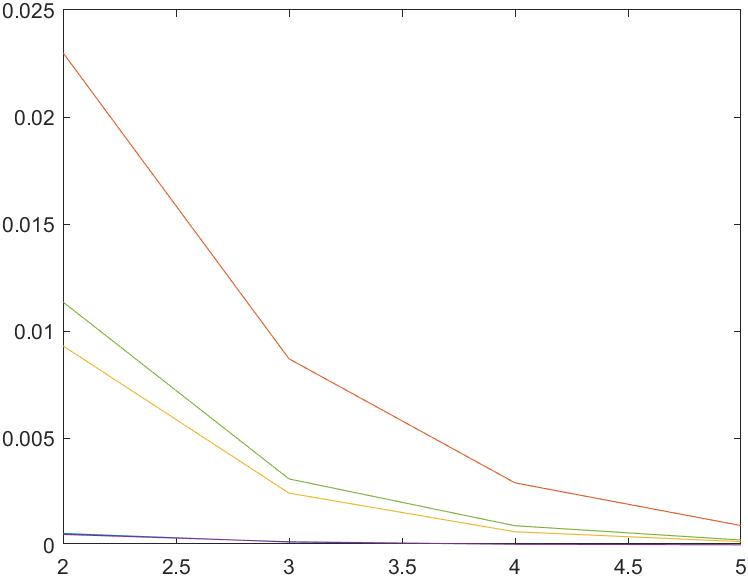
\includegraphics[scale=0.5]{1.jpg}$

画图代码见 m1.m。

另一例子的函数见注释,输出结果见 Dirichlet2.out 等文件。

\subsection{参考内容}

调用了 https://github.com/MikeMirzayanov/testlib 的 testlib 库。

\end{document}
